\documentclass[11pt, a4paper]{article}


\usepackage{anyfontsize}
\usepackage{txfonts} 
\usepackage{booktabs}
\usepackage{array}
\usepackage{geometry}
\usepackage{graphicx}
\graphicspath{{img/}}
\geometry{left=3cm,right=2.5cm,top=3.5cm,bottom=4cm}

%Graphics preamble
\usepackage{graphicx} %Allow you to import images
\usepackage{float} %Allow for control of float position

%Header and Footer Stuff
\pagestyle{myheadings}\markboth{page \thepage}{\emph Software Requirements Specification for 
Mesa Mapping Robot}

%Table
\setlength{\arrayrulewidth}{0.5mm}

\begin{document}

\begin{titlepage}

\begin{center}

	\vspace{0.5 cm}
	\fontsize{35}{35}\selectfont\bf {Software Requirements Specification}\\
	\vspace{0.5 cm}
	\huge{\bfseries for}\\
	\vspace{0.5 cm}
	\fontsize{35}{40}\selectfont\bf {Mesa Mapping Robot}\\
	
	\vspace{2cm}
	\Large\textbf{ Version 2.0 approved}\\
	
	\vspace{1.5cm}
	\Large\textbf {Prepared by SEP Group 19 - Spark\\
								Luo Yawen a1657343 \\
								Wei Jingwen a1671836 \\
								Wang Yuzhu a1690773 \\
								Yang Jiajun a1662541\\
								Zhang Yun a1653772 \\
								Zander Shaun Nathan a1146944}\\
		
	\vspace{2cm}
	\Large\textbf{ School of Computer Science,\\
								The University of Adelaide}\\
	\vspace{2cm}
	
	\Large\textbf{Nov 01, 2015}\\

\end{center}

\end{titlepage}

%This is table of contents stuff
\pagenumbering{roman}
\tableofcontents

%This is the version history stuff
\vspace{1cm}
\section*{Revision History}
\addcontentsline{toc}{section}{\numberline{}Revision History}
%\begin{table}
\small
\begin{tabular} 
	 {|m{3cm}|m{2cm}|m{8cm}|m{2cm}|}
	\hline
	\textbf{Name} &  \textbf{Date} & \textbf{Reason For Changes} & \textbf{Version} \\ [0.5ex]
	\hline
	Luo Yawen & 12/Aug/15 & Add the information of System Features & 0.1 \\ [0.5ex]
	\hline
	Yun Zhang & 13/Aug/15 & Add the information of System Features & 0.2 \\ [0.5ex]
	\hline
	Wang Yuzhu & 16/Aug/15 & Add the information of User requirements & 0.3 \\ [0.5ex]
	\hline
	Yang Jiajun & 17/Aug/15 & Add the information of User requirements & 0.4 \\ [0.5ex]
	\hline
	Wei Jingwen & 19/Aug/15 & Add the information of External Interface Requirements & 0.5 \\ [0.5ex]
	\hline
	Wei Jingwen & 20/Aug/15 & Add the information of Other Nonfunctional Requirements & 0.6 \\ [0.5ex]
	\hline
	Zander Shaun Nathan & 21/Aug/15 & Add Introduction & 0.7 \\ [0.5ex]
	\hline
	Wang Yuzhu & 22/Aug/15 & Add section 2.1 \& 2.2 \& 2.6 & 0.8 \\ [0.5ex]
	\hline
	Wei Jingwen & 22/Aug/15 & Add section 2.3 \& 2.4 & 0.9 \\ [0.5ex]
	\hline
	Yang Jiajun & 23/Aug/15 & Add section 2.5 \& 2.7 & 0.9.1 \\ [0.5ex]
	\hline
	Luo Yawen & 23/Aug/15 & Release & 1.0 \\ [0.5ex]
	\hline
	Wang Yuzhu & 27/Sep/15 & Update section 2.1 \& 2.2 \& 2.6 and 3 & 1.4 \\ [0.5ex]
	\hline
	Yang Jiajun & 28/Sep/15 & Update section 2.3 & 1.7 \\ [0.5ex]
	\hline
	Luo Yawen & 29/Sep/15 & Update section 4 \& figures of section 5 & 1.8 \\ [0.5ex]
	\hline
	Luo Yawen \newline  Wang Yuzhu \newline Yang Jiajun & 03/Oct/15 & Review & 1.9 \\ [0.5ex]
	\hline
	Luo Yawen & 01/Nov/15 & Final release & 2.0 \\ [0.5ex]
	\hline

\end{tabular}
%\end{table}
\cleardoublepage

\newpage


%This is main body stuff
\pagenumbering{arabic}
\setcounter{page}{1}

\section{Introduction}
\subsection{Purpose}
This document sets out the requirements for the Mesa Mapping Robot to be used for the Software Engineering and Project assignment for the University of Adelaide. Within this document, the primary requirements are set out for the Robot System which will be implemented in the second semester of 2015.\\
\\
Within this Software Requirements Specification (SRS) will be the description for the requirement of this system.

\subsection{Document Convention}
All user requirements will be given an code which will follow the convention Rnnnnn (n representing a number). Any deleted requirements will be labelled ``Requirement Deleted''. As any requirements are added they will be numbered sequentially therefore they will not be listed in ascending order in this document.\\
\\
User requirements will be allocated a priority. They will be labelled as either Low, Medium or High. High priority requirements must be implemented first and with the highest priority. Medium priority requirements are the next class of requirement and would be the good for the project to have but are not essential to the immediate use of the robot. However they may still need to be implemented in the long term use of the robot. Low priority requirements are non essential requirements and should only be implements if time allows it.

\subsection{Intended Audience and Reading Suggestions}
There are three categories of the audience for this document. Members of MesaMapping who are the client for the Mesa Mapping Project. PG19 who are the development team for the Mesa Mapping Project and the assessors of the Software Engineering and Project course.\\
\\
For the MesaMapping members, the intention of this document is for an agreement to be reached on the requirements and for further requirements to be given if required. MesaMapping clients should read the full document in order with particular detail to be given to User Requirements (Section 3) and Other Non-functional Requirements (Section 6).\\
\\
For the developers (PG19), the intention of this document is to provide detail for them to begin development of the software. Developers should read the full document in order with particular detail to be given to Other Non-functional Requirements (Section 6).\\
\\
For the assessors of the Software Engineering and Project course, the document should be read in full so that is can be included in the assessment of the group.

\subsection{Project Scope}
The software in this document is for the surveying of a Mesa to be done by a Lego Mindstorms EV3 robot. There are two main purposes of the software as laid out in this documents. The first is to conduct the safe execution of the navigation of the robot through the Mesa. The second is the accuracy of the mapping of the Mesa by the robot. Both tasks appear to be unrelated on the exterior however they are both integral to the implementation of the project and interrelated with one another.

\subsection{References}
Project Specification\\
https://forums.cs.adelaide.edu.au/pluginfile.php/46004/block/html/content/ProjectDescription/2015sem2.pdf\\
\\
SRS\_template\\
https://forums.cs.adelaide.edu.au/pluginfile.php/46014/mod/folder/content/0/SRS/template.pdf\\
\\
SRS Example\\
https://www.cise.ufl.edu/class/cen3031sp13/SRS/Example/1/2011.pdf

\section{Overall Description}
\subsection{Product Perspective}
The product described in this SRS describes is a new survey robot. Nowadays, map survey has been done by manual work. It is inefficiency, waste labor power and low accurate, particularly survey in a wide area. The new robot will be able to find markings which indicated by different colours and mark an accurate map according to the survey area automatically and can be moved smoothly from any point on the map to another. Also, the robot can continue working form where it left off. \\
\\
The map marked by the robot will show the location of the markings in the area of concern. The system is able to save the marked map, take an existing map file. The size of the survey area will determine the size of the map. 

\subsection{Product Features}
The main features of the robot include: \\
\begin{itemize}
\item Enable user to operate the robot.\\
The user is able to operate the robot by using the user interface, which includes the login screen, the main screen and the no-go zone (NGZ) set screen. The robot can be operated to turn left, turn right, go forward and go back smoothly. The user can operate the robot at all times. \\

\item Enable the user to stop the robot.\\
The user is able to instantly stop the robot by pushing the stop bottom in the main screen to stop the robot in case of emergency.\\

\item Enable the robot to survey the map automatically.\\
The base station is located in the centre of the survey area. There is a return to the base station function on the main screen. When the user pushes the return to the base station bottom, the robot is able to return to the base station automatically wherever the robot is.\\

\item Enable the robot to detect deposits.\\
The robot is able to find the deposit using the colour sensor. Deposits are indicated by different colours in the survey area and mark these colours.\\

\item Enable the robot to detect and mark the boundary.\\
The robot is able to detect and mark the boundary. The robot will stop before across the boundary. The boundary is rectangular, marked on the terrain with black solid line. There are black circles on the boundary before each corner.\\

\item Enable the robot to detect the NGZ.\\
The robot is able to detect the NGZ on the survey area. There is no visual representation of the NGZ on the survey area. There also is no uniform shape to the NGZ. NGZ is potential dangerous areas on the survey area, which the robot must not go.\\

\item Enable the user to load a map.\\
The user is able to load a map to the map area on the main screen. The size of the survey area determined the size of the map.\\

\item Enable the user to save the map.\\
The user is able to save the map. The system can save an existing map file, as the mapping process can take an amount time.\\
\end{itemize}

\subsection{User Classes and Characteristics}
In this project, for the robot there are two types of users including task manager and database recorder. Among them, the task manager is mainly responsible for initialing the task which includes setting up the boundary and no-go zone, as well as dealing with the emergency situation. As for the database recorder, this kind of user is required to save and record the maps that surveyed by the mapping robot.\\
\\
In addition, both of the users can only use the provided GUI to operate the robot. Any bug or unavailable function of the robot found when operating should be report immediately to the maintainers. Besides, any forms of adaptation to the software and hardware shall be and only be done by the robot maintainers. The robot maintainers also required to guarantee the required function work appropriately, and they shall be eligible with the ability to fix the potential problems (e.g. system breakdown, robot halt, software amendment, communication abort etc.). 

\subsection{Operating Environment}
The software will be installed on a MAC, supported by Lejos EV3 0.9.0 beta, Users shall be able to control the robot through the GUI which is operation friendly. The GUI shall able to be installed and be working under OS and windows PC.

\subsection{Design and Implementation Constraints}
The project involves the control of a Lego Mindstorms EV3 robot which will be programmed through leJOS software. After programming, the robot shall have the ability to detect and make a map of a certain area. \\
\\
Due to the risk and cost to allow a robot to operate on a real condition, for testing, a prototype will be utilized to this project. The prototype will be a paper/card which is no larger than A4 paper size.\\
\\
Some coloured circles would indicate the boundary and presence. For this reason, the robot?s operation will need to have an adjustment when applying to the real site.
The project will be programmed through JAVA. In addition to leJOS, Apache ant will also be used to develop the robot.

\subsection{User Documentation}
User manuals and on-line help will be made available to users. The user manual describes how to operate the robot, including turn left, turn right, move forward and move back, how to load and save maps and how to set the NGZ. The on-line help provides information about the operating system, the function of each button and help operators to solve problems quickly in case of emergency. 

\subsection{Assumptions and Dependencies}
We assume that we will take advantage of some JAVA API to program the robot. And the robot could be randomly assembled to satisfy the operation requirements. Furthermore, the robot can be operated manually through WIFI or Bluetooth.



\section{User Requirements}
This section describes the requirements for system users. Within this section the primary user requirements are sets out for the Mesa Mapping Robot System. Each requirement will be presented precisely, including description, rationale, criteria, dependencies and priority. 

\subsection{Operation}
\begin{itemize}
\item {\bfseries R0001: Start the Robot}\\
\textsc{\bfseries Description} The system shall support starting robot function for users. Users shall be able to start the robot at any time. No matter where the robot is.\\
\textsc{\bfseries Rationale} The system shall support starting robot function for users. Users shall be able to start the robot at any time. No matter where the robot is.\\
\textsc{\bfseries Priority} High\\

\item {\bfseries R0002: Stop the Robot}\\
\textsc{\bfseries Description} The system shall support the stopping the robot for users. Users shall be able to stop the robot at any time, no matter where the robot is. The stop function shall be used to stop the robot when the work finished, to stop the robot when any emergency happened, to stop the robot when users want to.\\
\textsc{\bfseries Rationale} Users should be able to stop the robot if the map has been completed or when is non-working time. Also, users should be able to stop the robot if there is an emergency.\\
\textsc{\bfseries Acceptance criteria} This requirement can be verified by pressing the stop button, then ensuring that the position of the robot on the map will not change and the robot will not have nay reaction even the user pressing the moving button.\\
\textsc{\bfseries Status} Implemented in initial prototype.\\
\textsc{\bfseries Priority} High\\

\item {\bfseries R0003: Return Base Station}\\
\textsc{\bfseries Description} The system shall support returning to base station function for users. Users shall be able to order the robot to return to base station at any time, no matter where the robot is. The base station will be allocated in the center of the map. The robot should be able to return to the base station automatically.\\
\textsc{\bfseries Rationale}Users should be able to order the robot to return to the base station when the robot finished the work or when the robot needs to be repaired. Also, users should be able to stop the robot if there is any emergency. This requirement will help users to operate the robot and reduce workload as the robot will return to the base station automatically.\\
\textsc{\bfseries Acceptance criteria} This requirement can be verified by pressing the return to the base button, then ensuring that the distance on the map between the robot and the base station, ensuring that the robot is moving back to the base station automatically.\\
\textsc{\bfseries Source} Based on the position of the robot and the base station.\\
\textsc{\bfseries Status} Implemented in initial prototype.\\
\textsc{\bfseries Priority} High\\

\item {\bfseries R0004: Automatic Operating}\\
\textsc{\bfseries Description} The system shall support the automatic operating function for users. Users shall be able to choose the automatic mode to make the robot working without manual operating. When the robot is in the automatic mode, the robot shall survey the map automatically including finding and marking markings, avoiding the NGZ and detecting and mapping the boundary.\\
\textsc{\bfseries Rationale}  Automatic operating will reduce manual operating and improve efficiency. The robot can survey the map without human control.\\
\textsc{\bfseries Acceptance criteria} This requirement can be verified by switching the working mode into automatic and pressing the start button, then ensuring that the robot is survey the map automatically, ensuring the robot can find and map the markings, ensuring that the robot will not enter the NGZ, ensuring that the robot will not accord the boundary.\\
\textsc{\bfseries Source} Based on the survey map.\\
\textsc{\bfseries Status} Implemented in initial prototype.\\
\textsc{\bfseries Priority} High\\

\item {\bfseries R0005: Manual Operating}\\
\textsc{\bfseries Description} The system shall support the manual operating function for users. Users shall be able to choose the manual mode to make the robot working in manual operating mode. When the robot is in the manual mode, the robot shall be controlled by users including start, stop, turning left, turning right, going forward and going back.\\
\textsc{\bfseries Rationale} Users should be able to operate the robot in manual mode in case of the automatic operating system error.\\
\textsc{\bfseries Acceptance criteria} This requirement can be verified by switching the working mode into manual and pressing the start button, then ensuring that the robot will be controlled by the user, ensuring that the robot will not move without the control of the user.\\
\textsc{\bfseries Source} Based on the survey map.\\
\textsc{\bfseries Status} Implemented in initial prototype.\\
\textsc{\bfseries Priority} High\\

\item {\bfseries R0006: Movement}\\
\textsc{\bfseries Description} The system shall support users to operate the robot to move on all sides, including turning left, turning right, going forward and going back.\\
\textsc{\bfseries Rationale} Users should be able to operate the to move on all sides, this will support the manual operating function.\\
\textsc{\bfseries Acceptance criteria} This requirement can be verified by pressing the control button on the user interface, ensuring that the robot will turn left when the user push the left button, ensuring that the robot will turn right when the user push the right button, ensuring that the robot will turn go forward when the user push the up button, ensuring that the robot will go back when the user push the down button.\\
\textsc{\bfseries Status} Implemented in initial prototype.\\
\textsc{\bfseries Priority} High\\
\end{itemize}

\subsection{Robot}
\begin{itemize}
\item {\bfseries R0007: Remaining Battery}\\
\textsc{\bfseries Description} The system shall support users to know the remaining battery of the robot. Users shall be able to know the remaining battery of the robot all the time. The remaining battery shall be presented on the user interface. There shall be an error message when the robot is in the low battery to remain the user.\\
\textsc{\bfseries Rationale} Users should be able to know the remaining battery, in order to estimate how long can the robot work for.\\
\textsc{\bfseries Acceptance criteria} This requirement can be verified by the battery area on the main user interface, the battery area will show the remaining battery of the robot.\\
\textsc{\bfseries Source} Based on the remaining battery of the robot.\\
\textsc{\bfseries Status} Implemented in initial prototype.\\
\textsc{\bfseries Priority} High\\

\item {\bfseries R0008: Show Current Position}\\
\textsc{\bfseries Description} The system shall support users to know the current position of the robot. Users shall be able to know the current position of the robot all the time. The current position of the robot shall be presented on the survey map.\\
\textsc{\bfseries Rationale} Users should be able to know the current position of the robot. This requirement will help users to know the position of the robot and help users to make next decision. This requirement will also help users to operate the robot and know the work progress.\\
\textsc{\bfseries Acceptance criteria} This requirement can be verified by moving the robot, ensuring that the position of the robot will change in the same time.\\
\textsc{\bfseries Source} Based on X and Y coordinates on the map.\\
\textsc{\bfseries Status} Implemented in initial prototype.\\
\textsc{\bfseries Priority} High\\

\item {\bfseries R0009: Information interaction}\\
\textsc{\bfseries Description} The system shall support the robot to sent message to the main user interface to communicate with users. As users shall know the situation of the robot all the time, including the status of the robot, the remaining battery, the condition of the working environment and the reason why the robot dose not move.\\
\textsc{\bfseries Rationale} Users should be able to know the status of the robot. This requirement will help users to know the status of the robot and help users to make next decision.\\
\textsc{\bfseries Acceptance criteria} This requirement can be verified by setting the robot into error status, ensuring that there is a corresponding message sent to the user.\\
\textsc{\bfseries Status} Implemented in initial prototype.\\
\textsc{\bfseries Priority} High\\
\end{itemize}

\subsection{Map}
\begin{itemize}
\item {\bfseries R0010: Load Survey Map}\\
\textsc{\bfseries Description}  The system shall provide the support for users loading the survey map on the system. Users shall be able to load survey map on the system. .\\
\textsc{\bfseries Rationale} Users should be able to load the survey map on the system. As users can operate the robot to survey the area according to the survey map.\\
\textsc{\bfseries Acceptance criteria} This requirement can be verified by pressing the map load button on the main user interface, ensuring that the chosen map can be presented on the map area on the main user interface.\\
\textsc{\bfseries Source} Based on existing map in the computer.\\
\textsc{\bfseries Status} Implemented in initial prototype.\\
\textsc{\bfseries Priority} High\\

\item {\bfseries R0011: Save Survey Map}\\
\textsc{\bfseries Description}The system shall provide the support for users saving the survey map. Users shall be able to save survey map from the system. The shall be able to saved, also, the map shall be saved as an existing file as the surveying process will take an amount of time.\\
\textsc{\bfseries Rationale} Users should be able to save the survey map to the computer. As the mapping process can take a plenty of time. This requirement should help the user to save the mapped and unmapped area, and help the robot to continue mapping from where if left off.\\
\textsc{\bfseries Acceptance criteria} This requirement can be verified by by pressing the map save button on the main user interface, ensuring that the surveyed map can be saved to the computer. When open the map, ensuring the markings are all on the map.\\
\textsc{\bfseries Source} Based on the surveyed map.\\
\textsc{\bfseries Status} Implemented in initial prototype.\\
\textsc{\bfseries Priority} High\\

\item {\bfseries R0012: Mark NGZ}\\
\textsc{\bfseries Description} The system shall provide the support for users setting NGZ on the survey map. Users shall be able to mark NGZ at any time. NGZ will either be pre defined or dynamically allocated. There will be no uniform shape and color to NGZ. They are the areas that the robot cannot go. \\
\textsc{\bfseries Rationale} Users should be able to mark NGZ on the survey map to restrict the robot enter the NGZ. As NGZ are potentially dangerous areas of the map, which the robot must not go.\\
\textsc{\bfseries Acceptance criteria} This requirement can be verified by setting the NGZ on the survey map, then operating the robot to this area, ensuring that the robot will stop before go into NGZ.\\
\textsc{\bfseries Source} Based on the survey map.\\
\textsc{\bfseries Status} Implemented in initial prototype.\\
\textsc{\bfseries Priority} High\\

\item {\bfseries R0013: Cancel NGZ}\\
\textsc{\bfseries Description} The system shall provide the support for users cancelling the NGZ on the survey map. Users shall be able to cancel NGZ at any time.\\
\textsc{\bfseries Rationale} The system shall provide the support for users cancelling the NGZ on the survey map. Users shall be able to cancel NGZ at any time.\\
\textsc{\bfseries Acceptance criteria} This requirement can be verified by pressing the NGZ clear button, ensuring that the chosen NGZ is disappeared on the survey map.\\
\textsc{\bfseries Source} Based on the exist NGZ on the map.\\
\textsc{\bfseries Status} Implemented in initial prototype.\\
\textsc{\bfseries Priority} High\\
\end{itemize}

\subsection{Authentication}
\begin{itemize}
\item {\bfseries R0014: Login Authentication}\\
\textsc{\bfseries Description} The system shall provide the authentication to users. Users will be required to login to the system using their through entering valid ID and password.\\
\textsc{\bfseries Rationale} For the reason of security, the robot will be operated only if the user is authorized. Unauthorized users should not be able to login to the robot and operate the robot.\\
\textsc{\bfseries Acceptance criteria} This requirement can be verified entering the user ID and password, ensuring that the valid user can login into the system and the invalid user can not login into the system.\\
\textsc{\bfseries Priority} Low\\

\item {\bfseries R0015: Restricted Login}\\
\textsc{\bfseries Description}  The system shall make sure that users should be only permitted to login to the system through their own ID information as well as valid password. It is forbidden to modify information of other users.\\
\textsc{\bfseries Rationale}Users should not have the capability to change others? information. This requirement can protect the system form maliciously attack.\\
\textsc{\bfseries Acceptance criteria} This requirement can be verified entering the user ID and password, ensuring that the valid user can login into the system and the invalid user can not login into the system, ensuring that users can only change their own information.\\
\textsc{\bfseries Priority} High\\

\item {\bfseries R0016: Logout}\\
\textsc{\bfseries Description} Users shall be able to logout the system after the end of operation. After logging out, unauthorized user shall not have the ability to operate the robot or modify related information. All system will expire after logging out.\\
\textsc{\bfseries Rationale}It is necessary to forbid the unauthorized user to operate the robot when previous user has logged the system.\\
\textsc{\bfseries Acceptance criteria} This requirement can be verified by logging the system, ensuring that users can not use the system, ensuring that users can use the system when log the system again.\\
\textsc{\bfseries Priority} High\\
\end{itemize}

\subsection{General}
\begin{itemize}
\item {\bfseries R0017: User Help} \\
\textsc{\bfseries Description} The system shall support the help function for users. Users shall be able to get help during the operation, including the explanation of every function of the robot, how to use every button on the screen and how to solve the error of robot.\\
\textsc{\bfseries Rationale} Users should be able to get help information from the system during the operation. Providing help information can help users to operate the robot better.\\
\textsc{\bfseries Acceptance criteria} This requirement can be verified by pressing the help button on the user interface or visiting the help information online.\\
\textsc{\bfseries Source} Based on the current support for the robot\\
\textsc{\bfseries Priority} High\\
\end{itemize}

\section{System Features}
This section describes the feature of system. Within this section the primary system requirements are based on the user requirements. Each requirement will be presented precisely, including description,  priority, basic flow and dependencies. 
\subsection{SF0001 Enter the survey map}
\textsc{\bfseries Description} The robot should be able to enter the survey area and produce the survey map.\\
\textsc{\bfseries Priority} 8\\
\textsc{\bfseries Basic Flow} \\
\textsc{E1:} Moving the robot to an initial starting position safely under manual control of the operator.\\
\textsc{E2:} Changing the state of robot to ready when it completes preparation.\\
\textsc{E3:} The control center takes over the control of the robot.\\
\textsc{E4:} The robot tells the control center its current position.\\

\subsection{SF0002 Saving map }
\textsc{\bfseries Description} The robot tells the control center its current position.\\
\textsc{\bfseries Priority} 6\\
\textsc{\bfseries Basic Flow} \\
\textsc{E1:} The control center commands the robot to save the current map.\\
\textsc{E2:} The robot saves the map into XML files.\\
\textsc{E3:} The robot tells the control center success of saving map.\\

\subsection{SF0003 Loading map}
\textsc{\bfseries Description} Loading the map from XML files.\\
\textsc{\bfseries Priority} 6\\
\textsc{\bfseries Basic Flow} \\
\textsc{E1:} The control center commands the robot to load the map locally or remotely.\\
\textsc{E2:} The robot downloads the map from control center if loading files remotely.\\
\textsc{E3:} Validating the XML file against the DTD file.\\
\textsc{E4:} Loading and transforming the file.\\

\subsection{SF0004 Moving robot smoothly}
\textsc{\bfseries Description} The robot should move to destination specified by the control center.\\
\textsc{\bfseries Priority} 8\\
\textsc{\bfseries Basic Flow} \\
\textsc{E1:} The control center commands the robot to move to destination specified by the control center.\\
\textsc{E2:} The robot should move to destination at a stable speed.\\

\subsection{SF0005 NGZ specifications}
\textsc{\bfseries Description} The control center should specify the no-go zone where the robot should not enter. Assume the NGZ is rectangular.\\
\textsc{\bfseries Priority} 9\\
\textsc{\bfseries Basic Flow} \\
\textsc{E1:} The control center specifies the NGZ by using a pair of coordinates.\\
\textsc{E2:} E2: The robot should not enter the NGZ.\\

\subsection{SF0006 Boundary detection and marking}
\textsc{\bfseries Description} The map should have boundary that the robot cannot enter, and the robot should mark it when the robot detects it.\\
\textsc{\bfseries Priority} 9\\
\textsc{\bfseries Basic Flow} \\
\textsc{E1:} The control center should tell the robot the color of the boundary lines.\\
\textsc{E2:} The robot should stop when it detects the boundary lines.\\

\subsection{SF0007 Deposit detection}
\textsc{\bfseries Description} The map should have deposits that the robot cannot touch, and the robot should mark them when the robot detects them.\\
\textsc{\bfseries Priority} 9\\
\textsc{\bfseries Basic Flow} \\
\textsc{E1:} The control center should tell the robot the colors of the circles.\\
\textsc{E2:} The robot should bypass or stop when it detects the circles.\\

\subsection{SF0008 Tower and base detection and marking}
\textsc{\bfseries Description} The map should have communications tower and operations base, and the robot should mark them when the robot detects them.\\
\textsc{\bfseries Priority} 8\\
\textsc{\bfseries Basic Flow} \\
\textsc{E1:} The control center should tell the robot the characteristics of the communications tower and operations base.\\
\textsc{E2:} The robot should mark the buildings when it finds them.\\

\subsection{SF0009 Robot stays in the boundary}
\textsc{\bfseries Description} The robot should focus its position, stay in the boundary and cannot cross it.\\
\textsc{\bfseries Priority} 9\\
\textsc{\bfseries Basic Flow} \\
\textsc{E1:} The robot should use its color sensor to detect the position of boundary.\\
\textsc{E2:} If the robot touches the boundary, it needs to stop immediately.\\
\textsc{E3:} The robot cannot across the boundary and keep itself inside the boundary.\\

\subsection{SF0010 Robot Avoids collision}
\textsc{\bfseries Description} The robot should detect environment accurately to avoid collision.\\
\textsc{\bfseries Priority} 9\\
\textsc{\bfseries Basic Flow} \\
\textsc{E1:} The robot should slow down when it detects an obstacle using its distance sensor.\\
\textsc{E2:} The robot should bypass the detected objects.\\

\subsection{SF0011 Stop automatically}
\textsc{\bfseries Description} When the communication is lost, the robot should stop automatically.\\
\textsc{\bfseries Priority} 9\\
\textsc{\bfseries Basic Flow} \\
\textsc{E1:} The communication between the robot and the control center is lost.\\
\textsc{E2:} The robot should stop immediately.\\
\newpage

\section{External Interface Requirements}
\subsection{User Interfaces}
Users will interface with the Robot through a Graphical User Interface (GUI). The GUI shall use visible button to indicate available function that the robot able to execute. The quantitative action shall also have blanks for users to fill in. In addition, the auto-manual switch shall also have distinct interface which will facilitate user observe mode easily. The status of the robot will be display on the GUI which includes coordinates communicate messages and state of charge.

%Here we insert our figure
\begin{figure}[H]
\centering
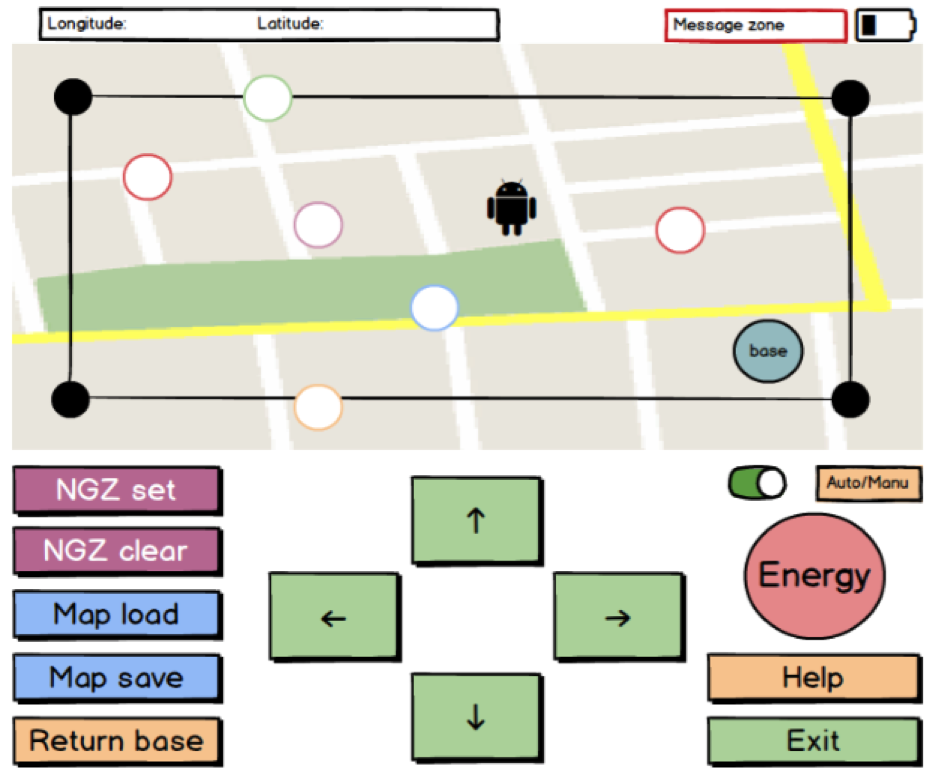
\includegraphics[height=3in]{MainInterface1}
\caption[Main Interface]{Main Interface1}
\end{figure}

\begin{figure}[H]
\centering
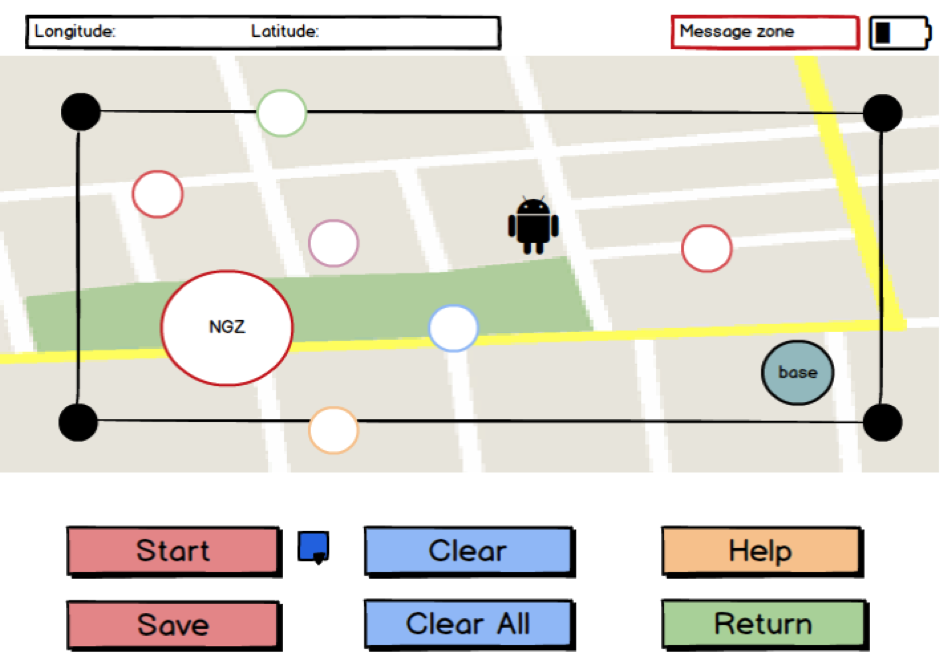
\includegraphics[height=3in]{MainInterface2}
\caption[Main Interface]{Main Interface2}
\end{figure}

\subsection{Hardware Interfaces}
The robot consists with a main dynamical system, sensor system and processing and communication system. Firstly, Main dynamical system consists of two large motors, and a medium motor, as the robot use crawler instead of wheel the dynamical system shall enable robot accomplish forward, backward, turning etc. Additionally, the medium motor used for adapting the position of sensors as well as the head. Secondly, the sensor system has four types of sensor, which are touch sensor, colour sensor, bump sensor and ultrasonic sensor. In this specific case touch sensor shall be an obstacle finder, which placed in front of the robot and halt the robot immediately after trigger. Colour sensor and ultrasonic sensor is placed in the arms of the robot, which helps the robot identify the colour and objects. Bump sensor was placed in the back of the robot which assist the robot acknowledges the situation while turning. Thirdly, the processing and communication are accomplished in the Lego EV3 brick.

\subsection{Software Interfaces}
The software interface includes the GUI.  However despite of the manual function, which was displayed in GUI, an Application Programming Interface (API) is provided for making action plan. The robot programming was based on Java versioned 1.6.0\_65. The robot sensor protocols are from LEGO, and the leJOS\_EV3\_0.9.0 beta is for the robot.
%Here we insert our figure
\begin{figure}[H]
\centering
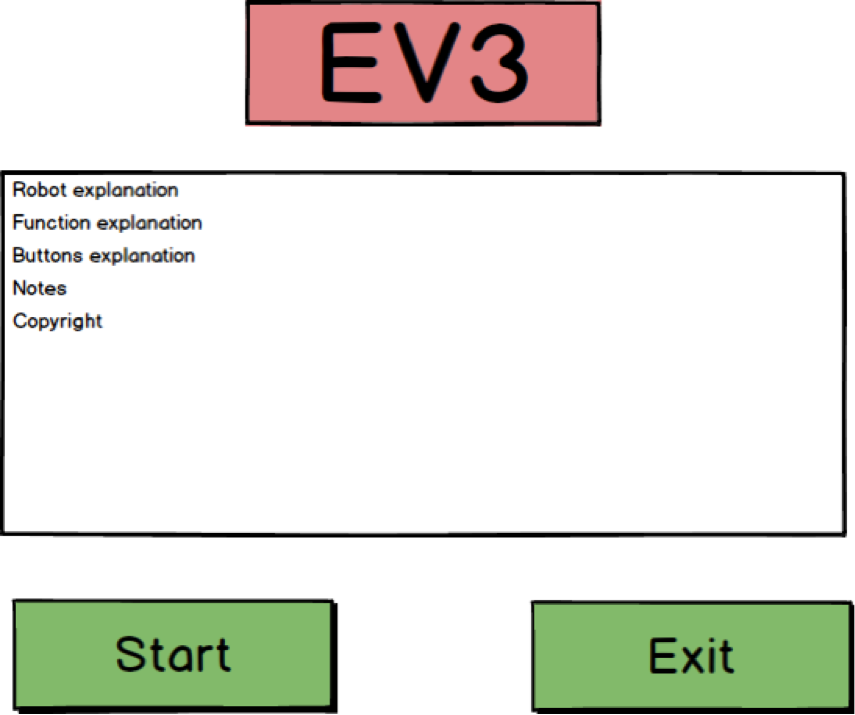
\includegraphics[height=3in]{PI}
\caption[Application Programming Interface]{Application Programming Interface}
\end{figure}

\subsection{Communications Interfaces}
The communication between the robot and the user shall connecting with Wi-Fi, and the communication mission shall bond tightly with users PC and real-time. Anytime lose inter-face will cause the halt of the robot until the reconnection has accomplished.

\section{Other Nonfunctional Requirements}
\subsection{Performance Requirements}
The constraints on the robot services would be under these rules.  Firstly, the robot shall be working in the boundary: the boundary includes the boundary of the map and the no-go zone (NGZ), which defined before and after the robot automatically working.  Secondly, the security of the robot shall consider as the top priority any action that may cause the damage to the robot shall be prevented. Thirdly, the robot shall able to accomplish the mission with the highest capable speed.

%\subsection{Safety Requirements}

\subsection{Security Requirements}
The security of the robot shall consider as the top priority of the robot, so any actions or commands that against the safety of the robot shall be cancelled and notifying the user.  The boundary of the map as well as the user-defined NGZ are recognized as dangerous to the robot as well shall be identified automatically by the robot and prevent from go through as well.  Additionally, any type of lose communication with user PC shall be treated as a potentially dangerous signal therefore the robot shall halt and save all remained action and wait for re-connection.

\subsection{Software Quality Attributes}
Availability of System is determined by both the user and the robot team, the user shall able to real-time control robot (Caution: the robot do not turn on the detect mode while manual mode, User shall be responsible for the robot security when operating the robot).  In addition, user is authorized some programmable actions for the robot, it is controlled in fixed range in order to avoid the potential damage to the robot.\\    
\\
The automatic mapping mode shall enable the robot to detect the outline and the over view of an area.  The low speed and stop may occur while encounter the boundary NGZ and obstacle but the software shall able to find way to solve the possible situation and continue the asserted task. However, if the situation is unable to solve itself, the robot shall inform the user and halt for the further instruction.

%\section{Other Requirements}

%Appendix
\section*{Appendix A: Glossary}
\addcontentsline{toc}{section}{\numberline{}Appendix A: Glossary}
\begin{itemize}
\item {PC - }Personal Computer\\
\item {API - }Application Programming Interface\\
\item {DTD - }Document Type Definition\\
\item {XML - }Extensible Markup Language\\
\item {SRS - }Software Requirement Specification\\
\item {NGZ - }No-go Zones\\
\item {GUI - }Graphic User Interface\\
\end{itemize}

\end{document}